\documentclass[14pt,a4paper,russian]{article}
% \documentclass[14pt,a4paper]{extarticle}
\usepackage[14pt]{extsizes}
\usepackage[utf8]{inputenc} 
\usepackage[T2A]{fontenc} % before babel!
\usepackage[english, russian]{babel}
\usepackage[titletoc]{appendix}
\usepackage{amsmath}
\usepackage{amssymb}
\usepackage{bm}
\usepackage{babel,blindtext}  
\usepackage[backend=bibtex,style=numeric]{biblatex}  %backend=biber is 'better'  


%\usepackage{polyglossia}


\usepackage{caption}
\usepackage{color}
\usepackage{epigraph}
\usepackage{epsfig}
\usepackage{float}
\usepackage{textcomp}
\usepackage{gensymb}
\usepackage{graphicx}
\usepackage{hyperref}   
\usepackage{mathtools}
\usepackage{lipsum}
\usepackage{indentfirst,latexsym}
\usepackage{physics}
\usepackage{setspace}
\usepackage{subcaption}

\graphicspath{{img/}}

\addbibresource{kursach.bib}
%\selectlanguage{russian}

\onehalfspacing

%\usepackage{fontspec}
%\usepackage{polyglossia}
%\setmainfont[Ligatures=TeX]{cmunrm.otf}
%% \setmainfont[Ligatures=NoCommon]{Times New Roman}
%\setmainlanguage{russian}
%\setotherlanguage{english}
%\newfontfamily\cyrillicfonttt{lmmonolt10-bold.otf}


%% \newcommand{\be}{\begin{equation}}
%% \newcommand{\ee}{\end{equation}}
%% newcommand{\df} {\mathop{}\!\mathrm{d}}


\textheight 25.7cm % 29.7-2-2=25.7
\textwidth 17cm % 21-2.5-1.5=17.0
\hoffset -0.04cm %2.5-2.54=-0.04 слева 3см
\voffset -1.04cm %2-2.54=0.54 сверху 2см
\oddsidemargin 0cm
\headheight 0cm
\headsep 0cm
\topmargin 0cm
\setcounter{page}{1}
\def\sigspace{\\[1em]
\underline{\hspace{5cm}}\\[-0.2em]}




\begin{document}

\begin{titlepage}
	\begin{center}
		{
		{\bf Санкт-Петербургский Государственный Университет\\
		\vskip 1em
		Математико-механический факультет\\
		Кафедра Астрономии} }

	\vspace{3cm}
    	
	{\large А.С.\,Патшин}
    
    \vskip 2em
    

	\Large{\bf{Сравнение тригонометрических параллаксов звезд TGAS и Hipparcos}}
    \vskip 1em
    {\normalsize {Дипломная работа}\\}
	\end{center}
	
	\vskip 5em
    
	{
		 \begin{flushright}
			Научный руководитель:\\
		    доцент А.С.\,Цветков\sigspace
		    Рецензент:\\
		    PhD. З.М.\,Малкин\sigspace
		\end {flushright}
	}

	\vfill
	\begin{center}
	\small {Санкт-Петербург

	2018}
	\end{center}
\end{titlepage}

\newpage
\begin{titlepage}
	\begin{center}
		{
		{\bf Saint-Petersburg State University\\
		\vskip 1em
		Mathematics and Mechanics Department\\
		Chair of Astronomy} }

	\vspace{3cm}
    	
	{\large Anton Patshin}
    
    \vskip 2em
    

	\Large{\bf{Comparison of trigonometric parallaxes of TGAS and Hipparcos stars}}
    \vskip 1em

    {\normalsize {Graduation Thesis}\\}
	\end{center}
	
	\vskip 5em
    
	{
		 \begin{flushright}
			Scientific supervisor:\\
		    associate professor Alexander Tsvetkov\sigspace
		    Reviewer:\\
		    PhD. Zinovy Malkin \sigspace
		    
		\end {flushright}
	}

	\vfill
	\begin{center}
	\small {Saint-Petersburg

	2018}
	\end{center}
\end{titlepage}
\newpage
\tableofcontents
\newpage



 
\section{Введение}\label{introduction}

Сравнение каталогов является класической задачей фундаментальной астрометрии, производщей переход от отдной системы координат к другой, оценить уровень систематических ошибок. До недавненго времени могло проводиться сравнение лишь положений и собственных движений.Появление первых результатов миссии GAIA, в частности, каталога TGAS, позволило впервые проихвести сравение тригонометрических параллаксов общих звезд каталогов TGAS и  Hipparcos, а именно его второй версии XHIP (XHIP: An extended hipparcos compilation, Anderson, 2012). Каталог TGAS содержит 2057050 звезд с данными о тригонометрических параллаксах, включает в себя только звезды Hipparcos и Tycho-2  и не является в полном смысле независимым продуктом, т.к. использует в качестве первой эпохи данные этих двух каталогов. Для сравнения мы используем общие звезды XHIP  и TGAS, которых оказалось 93635, из которыз пригодно для анализа 90282.

\subsection{Общие сведенья о GAIA и TGAS}\label{sub:smthgaia}
Каталог GAIA
		
\subsection{Общие сведенья о Hipparcos}\label{sub:smthhip}
Тут мой супер классный диплом

\subsection{Постановка задачи}\label{sub:smthzd}
	Сравнение параллаксов.\\
Возможно два варианта, что подобные результаты могут быть случайными выбросами или систематическими разностями. нгн
			 
\section{Случайные выбросы}\label{errvid}

\subsection{Распределение}\label{sub:smthrs}
Тут мой супер классный диплом

\section{Систематические различия}\label{sistem}
		
\subsection{Healpix}\label{sub:smthhealpix}
HealPix -- это абревиатура \textbf{H}ierarchical \textbf{E}qual \textbf{A}rea iso\textbf{L}atitude \textbf{Pix}elation of a sphere (Иерархическая равная изоляционная площадь пикселей). Как бло предложено в названии, эта пикселизация создаёт сигменты сферической поверхности, в которой каждый пиксель покрывает ту же площадь поверхности, что и каждый другой пиксель.

Вся сфера делится на 12 равных по площади сигментов, как показано на правой верхнем рисунке ~\ref{img:healpix}. Последующее деление проиходит за счёт деления каждого имеющегося сигмента на 4 части. За счёт чего мы можем получить очень мелкое разбиение. 

HealPix имеет два режима резбиения:

\* нест - позволяет работать со сферическими функциями

\* не нест - позволяет определять минимальное расстояние до точек.

Мы будем использовать нест.

\begin{figure}[h!]
\center{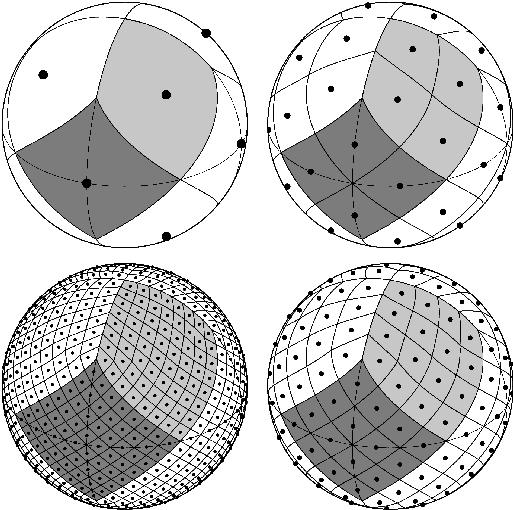
\includegraphics[width=0.5\linewidth]{healpix}}
\caption{Деление сферы на равные по пложади сигменты.}
\label{img:healpix}
\end{figure}

~\cite{wiki:healpix} 


\subsection{Сферические функции}\label{sub:smthsf}
Сферичекие функции очень полезный инстуррумент при анализе небесной сферы ~\ref{img:sf} .
~\cite{book:sf}

\begin{figure}[h!]
\center{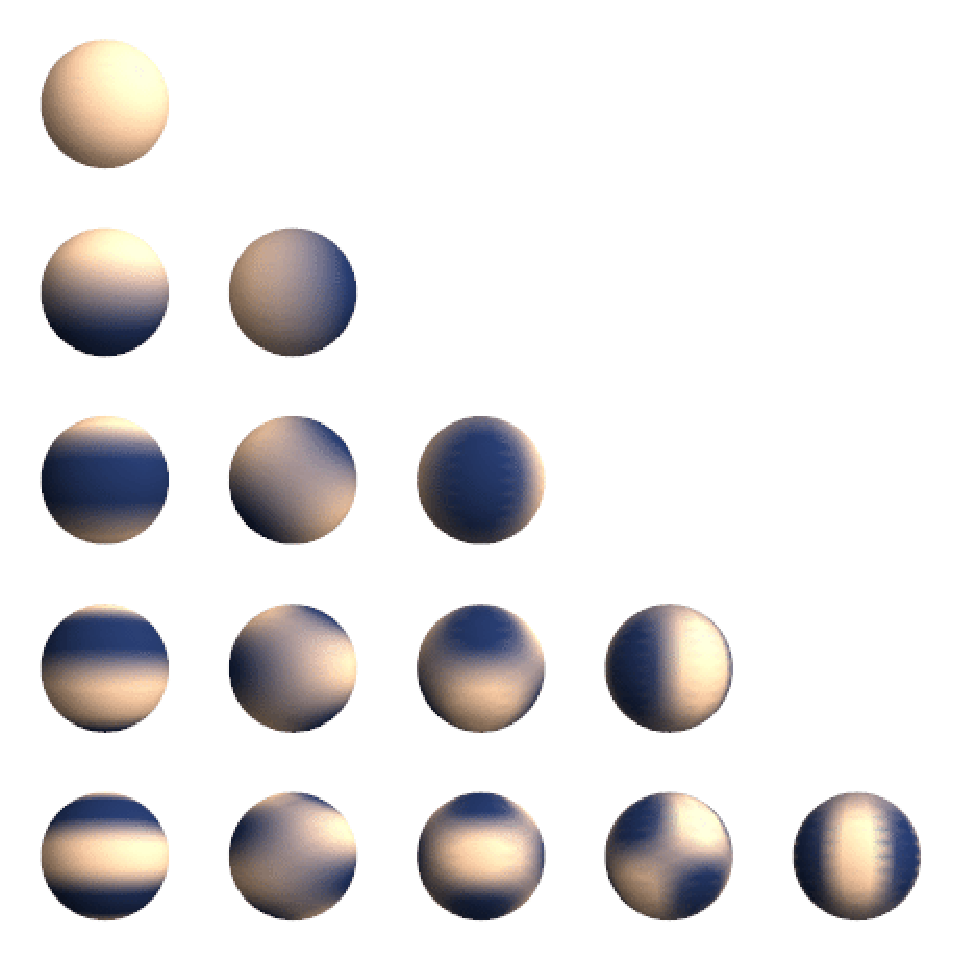
\includegraphics[width=0.5\linewidth]{Rotating_spherical_harmonics-0}}
\caption{Вещественные сферические функции $Y_{lm}$, $l=0…4$ (сверху вниз), $m=0…4$ (слева направо). Функции отрицательного порядка $Y_{l-m}$ повёрнуты вокруг оси Z на 90/m градусов относительно функций положительного порядка.}
\label{img:sf}
\end{figure}



\section{Заключение}\label{conclusion}
		ну вот и всё \cite{book:fourier} 

\newpage
\section{Список использованной литературы}\label{conclusionlit}
%\bibliographystyle{unsrt}
%\bibliography{kursach.bib}
\printbibliography[type=online,title={Online only}]
\printbibliography[type=book,title={Статьи:}]


\appendix

\section*{Приложение}
тут аппендикс или два 

\end{document}

